\hypertarget{bioenergetics}{%
\chapter{Bioenergetics}\label{bioenergetics}}

\href{https://en.wikipedia.org/wiki/Bioenergetics}{Bioenergetics} is a field in biochemistry and cell biology that concerns energy flow through living systems. This is an active area of biological research that includes the study of the transformation of energy in living organisms and the study of thousands of different cellular processes such as cellular respiration and the many other metabolic and enzymatic processes that lead to production and utilization of energy in forms such as adenosine triphosphate (ATP) molecules. That is, the goal of bioenergetics is to describe how living organisms acquire and transform energy in order to perform biological work. The study of metabolism and metabolic pathways is thus essential to bioenergetics.

The ability to harness energy from a variety of metabolic pathways is a property of all living organisms that contains earth science. Growth, development, anabolism and catabolism are some of the central processes in the study of biological organisms, because the role of energy is fundamental to such biological processes. Life is dependent on energy transformations; living organisms survive because of exchange of energy between living tissues/ cells and the outside environment. Some organisms, such as autotrophs, can acquire energy from sunlight (through photosynthesis) without needing to consume nutrients and break them down. Other organisms, like heterotrophs, must intake nutrients from food to be able to sustain energy by breaking down chemical bonds in nutrients during metabolic processes such as glycolysis and the citric acid cycle. Importantly, as a direct consequence of the first law of thermodynamics, autotrophs and heterotrophs participate in a universal metabolic network---by eating autotrophs (plants), heterotrophs harness energy that was initially transformed by the plants during photosynthesis.

In a living organism, chemical bonds are broken and made as part of the exchange and transformation of energy. Energy is available for work (such as mechanical work) or for other processes (such as chemical synthesis and anabolic processes in growth), when weak bonds are broken and stronger bonds are made. The production of stronger bonds allows release of usable energy.

Adenosine triphosphate (ATP) is the main ``energy currency'' for organisms; the goal of metabolic and catabolic processes are to synthesize ATP from available starting materials (from the environment), and to break- down ATP (into adenosine diphosphate (ADP) and inorganic phosphate) by utilizing it in biological processes. In a cell, the ratio of ATP to ADP concentrations is known as the ``energy charge'' of the cell. A cell can use this energy charge to relay information about cellular needs; if there is more ATP than ADP available, the cell can use ATP to do work, but if there is more ADP than ATP available, the cell must synthesize ATP via oxidative phosphorylation.



\begin{figure}

{\centering 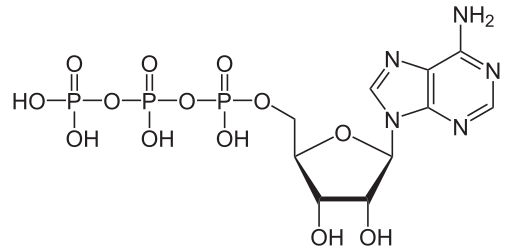
\includegraphics[width=0.7\linewidth]{./figures/bioenergetics/Adenosintriphosphat_protoniert} 

}

\caption{\href{https://commons.wikimedia.org/wiki/File:Adenosintriphosphat_protoniert.svg}{Structure of adenosine triphosphate (ATP), protonated}}\label{fig:atpstrucform}
\end{figure}

Living organisms produce ATP from energy sources, mostly sunlight or O2, mainly via oxidative phosphorylation. The terminal phosphate bonds of ATP are relatively weak compared with the stronger bonds formed when ATP is hydrolyzed (broken down by water) to adenosine diphosphate and inorganic phosphate. Here it is the thermodynamically favorable free energy of hydrolysis that results in energy release; the phosphoanhydride bond between the terminal phosphate group and the rest of the ATP molecule does not itself contain this energy. An organism's stockpile of ATP is used as a battery to store energy in cells. Utilization of chemical energy from such molecular bond rearrangement powers biological processes in every biological organism.

Living organisms obtain energy from organic and inorganic materials; i.e.~ATP can be synthesized from a variety of biochemical precursors. For example, lithotrophs can oxidize minerals such as nitrites or forms of sulfur, such as elemental sulfur, sulfites, and hydrogen sulfide to produce ATP. In photosynthesis, autotrophs produce ATP using light energy, whereas heterotrophs must consume organic compounds, mostly including carbohydrates, fats, and proteins. The amount of energy actually obtained by the organism is lower than the amount released in combustion of the food; there are losses in digestion, metabolism, and thermogenesis.

Environmental materials that an organism intakes are generally combined with oxygen to release energy, although some can also be oxidized anaerobically by various organisms. The bonds holding the molecules of nutrients together and in particular the bonds holding molecules of free oxygen together are relatively weak compared with the chemical bonds holding carbon dioxide and water together. The utilization of these materials is a form of slow combustion because the nutrients are reacted with oxygen (the materials are oxidized slowly enough that the organisms do not actually produce fire). The oxidation releases energy because stronger bonds (bonds within water and carbon dioxide) have been formed. This net energy may evolve as heat, which may be used by the organism for other purposes, such as breaking other bonds to do chemistry required for survival.

\hypertarget{thermodynamics-of-living-organisms}{%
\section{Thermodynamics of Living Organisms}\label{thermodynamics-of-living-organisms}}

Thermodynamics is a branch of physics that deals with heat, work, and temperature, and their relation to energy, radiation, and properties of matter. The behavior of these quantities is governed by the four laws of thermodynamics which convey a quantitative description using measurable macroscopic physical quantities, but may be explained in terms of microscopic constituents by statistical mechanics.

Historically, thermodynamics developed out of a desire to increase the efficiency of early steam engines, particularly through the work of French physicist \href{https://en.wikipedia.org/wiki/Nicolas_Léonard_Sadi_Carnot}{Nicolas Léonard Sadi Carnot} (1824) who believed that engine efficiency was the key that could help France win the Napoleonic Wars. Scots-Irish physicist \href{https://en.wikipedia.org/wiki/William_Thomson,_1st_Baron_Kelvin}{William Thomson} (Lord Kelvin) was the first to formulate a concise definition of thermodynamics in 1854 which stated, ``Thermo-dynamics is the subject of the relation of heat to forces acting between contiguous parts of bodies, and the relation of heat to electrical agency.''

The initial application of thermodynamics to mechanical heat engines was quickly extended to the study of chemical compounds and chemical reactions. Biological thermodynamics is the quantitative study of the energy transductions that occur in or between living organisms, structures, and cells and of the nature and function of the chemical processes underlying these transductions. Biological thermodynamics may address the question of whether the benefit associated with any particular phenotypic trait is worth the energy investment it requires.

Living organisms must obey the laws of thermodynamics, which describe the transfer of heat and work. The First Law of Thermodynamics is a statement of the conservation of energy; though it can be changed from one form to another, energy can be neither created nor destroyed. The Second Law of Thermodynamics is concerned primarily with whether or not a given process is possible. The Second Law states that no natural process can occur unless it is accompanied by an increase in the entropy of the universe. Stated differently, an isolated system will always tend to disorder. Although living organisms' amazing complexity appears to contradict this law, life is possible as all organisms are open systems that exchange matter and energy with their surroundings. Thus living systems are not in equilibrium, but instead are dissipative systems that maintain their state of high complexity by causing a larger increase in the entropy of their environments. The metabolism of a cell achieves this by coupling the spontaneous processes of catabolism to the non-spontaneous processes of anabolism. In thermodynamic terms, metabolism maintains order by creating disorder.

As the environments of most organisms are constantly changing, the reactions of metabolism must be finely regulated to maintain a constant set of conditions within cells, a condition called homeostasis. Metabolic regulation also allows organisms to respond to signals and interact actively with their environments. Two closely linked concepts are important for understanding how metabolic pathways are controlled. Firstly, the regulation of an enzyme in a pathway is how its activity is increased and decreased in response to signals. Secondly, the control exerted by this enzyme is the effect that these changes in its activity have on the overall rate of the pathway (the flux through the pathway). For example, an enzyme may show large changes in activity (i.e.~it is highly regulated) but if these changes have little effect on the flux of a metabolic pathway, then this enzyme is not involved in the control of the pathway.

There are multiple levels of metabolic regulation. In intrinsic regulation, the metabolic pathway self-regulates to respond to changes in the levels of substrates or products; for example, a decrease in the amount of product can increase the flux through the pathway to compensate. This type of regulation often involves allosteric regulation of the activities of multiple enzymes in the pathway. Extrinsic control involves a cell in a multicellular organism changing its metabolism in response to signals from other cells. These signals are usually in the form of water soluble messengers such as hormones and growth factors and are detected by specific receptors on the cell surface. These signals are then transmitted inside the cell by second messenger systems that often involved the phosphorylation of proteins.

A very well understood example of extrinsic control is the regulation of glucose metabolism by the hormone insulin. Insulin is produced in response to rises in blood glucose levels. Binding of the hormone to insulin receptors on cells then activates a cascade of protein kinases that cause the cells to take up glucose and convert it into storage molecules such as fatty acids and glycogen. The metabolism of glycogen is controlled by activity of phosphorylase, the enzyme that breaks down glycogen, and glycogen synthase, the enzyme that makes it. These enzymes are regulated in a reciprocal fashion, with phosphorylation inhibiting glycogen synthase, but activating phosphorylase. Insulin causes glycogen synthesis by activating protein phosphatases and producing a decrease in the phosphorylation of these enzymes.

The central pathways of metabolism described below, such as glycolysis and the citric acid cycle, are present in all three domains of living things and were present in the last universal common ancestor. This universal ancestral cell was prokaryotic and probably a methanogen that had extensive amino acid, nucleotide, carbohydrate and lipid metabolism. The retention of these ancient pathways during later evolution may be the result of these reactions having been an optimal solution to their particular metabolic problems, with pathways such as glycolysis and the citric acid cycle producing their end products highly efficiently and in a minimal number of steps. The first pathways of enzyme-based metabolism may have been parts of purine nucleotide metabolism, while previous metabolic pathways were a part of the ancient RNA world.

Many models have been proposed to describe the mechanisms by which novel metabolic pathways evolve. These include the sequential addition of novel enzymes to a short ancestral pathway, the duplication and then divergence of entire pathways as well as the recruitment of pre-existing enzymes and their assembly into a novel reaction pathway. The relative importance of these mechanisms is unclear, but genomic studies have shown that enzymes in a pathway are likely to have a shared ancestry, suggesting that many pathways have evolved in a step-by-step fashion with novel functions created from pre-existing steps in the pathway. An alternative model comes from studies that trace the evolution of proteins' structures in metabolic networks, this has suggested that enzymes are pervasively recruited, borrowing enzymes to perform similar functions in different metabolic pathways. These recruitment processes result in an evolutionary enzymatic mosaic. A third possibility is that some parts of metabolism might exist as ``modules'' that can be reused in different pathways and perform similar functions on different molecules.

As well as the evolution of new metabolic pathways, evolution can also cause the loss of metabolic functions. For example, in some parasites metabolic processes that are not essential for survival are lost and preformed amino acids, nucleotides and carbohydrates may instead be scavenged from the host. Similar reduced metabolic capabilities are seen in endosymbiotic organisms.



\begin{figure}

{\centering \includegraphics[width=0.7\linewidth]{./figures/bioenergetics/Sun_in_February_black_version} 

}

\caption{\href{https://commons.wikimedia.org/wiki/File:Sun_in_February_(black_version).jpg}{The Sun} is the source of energy for most of life on Earth. It derives its energy mainly from nuclear fusion in its core, converting mass to energy as protons are combined to form helium. This energy is transported to the sun's surface then released into space mainly in the form of radiant (light) energy.}\label{fig:energyfromsun}
\end{figure}

The sun is the primary source of energy for living organisms on earth. The relationship between the energy of the incoming sunlight and its wavelength λ or frequency ν is given by

\[ E={\frac  {hc}{\lambda }}=h\nu \]

where h is the Planck constant (6.63x10\textsuperscript{−34}Js) and c is the speed of light (2.998x10\^{}8 m/s). Plants trap this energy from the sunlight and perform photosynthesis, effectively converting solar energy into chemical energy. To transfer the energy once again, animals will feed on plants (or other animals) and use the energy of digested plant (or animal) materials to create biological macromolecules.

Energy flow, also called the calorific flow, refers to the flow of energy through a food chain.

A general energy flow scenario follows:

\begin{itemize}
\tightlist
\item
  Solar energy is fixed by the photoautotrophs, called primary producers, like green plants. Primary consumers absorb most of the stored energy in the plant through digestion, and transform it into the form of energy they need, such as adenosine triphosphate (ATP), through respiration. A part of the energy received by primary consumers, herbivores, is converted to body heat (an effect of respiration), which is radiated away and lost from the system. The loss of energy through body heat is far greater in warm-blooded animals, which must eat much more frequently than those that are cold-blooded. Energy loss also occurs in the expulsion of undigested food (egesta) by excretion or regurgitation.
\item
  Secondary consumers, carnivores, then consume the primary consumers, although omnivores also consume primary producers. Energy that had been used by the primary consumers for growth and storage is thus absorbed into the secondary consumers through the process of digestion. As with primary consumers, secondary consumers convert this energy into a more suitable form (ATP) during respiration. Again, some energy is lost from the system, since energy which the primary consumers had used for respiration and regulation of body temperature cannot be utilized by the secondary consumers.
\item
  Tertiary consumers, which may or may not be apex predators, then consume the secondary consumers, with some energy passed on and some lost, as with the lower levels of the food chain.
\item
  A final link in the food chain are decomposers which break down the organic matter of the tertiary consumers (or whichever consumer is at the top of the chain) and release nutrients into the soil. They also break down plants, herbivores and carnivores that were not eaten by organisms higher on the food chain, as well as the undigested food that is excreted by herbivores and carnivores. Saprotrophic bacteria and fungi are decomposers, and play a pivotal role in the nitrogen and carbon cycles.
\end{itemize}

The energy is passed on from trophic level to trophic level and each time about 90\% of the energy is lost, with some being lost as heat into the environment (an effect of respiration) and some being lost as incompletely digested food (egesta). Therefore, primary consumers get about 10\% of the energy produced by autotrophs, while secondary consumers get 1\% and tertiary consumers get 0.1\%. This means the top consumer of a food chain receives the least energy, as much of the food chain's energy has been lost between trophic levels. This loss of energy at each level limits typical food chains to only four to six links.

\hypertarget{metabolism}{%
\section{Metabolism}\label{metabolism}}

Metabolism (from Greek: μεταβολή metabolē, ``change'') is the set of life-sustaining chemical reactions in organisms. The three main purposes of metabolism are: the conversion of food to energy to run cellular processes; the conversion of food/fuel to building blocks for proteins, lipids, nucleic acids, and some carbohydrates; and the elimination of nitrogenous wastes. These enzyme-catalyzed reactions allow organisms to grow and reproduce, maintain their structures, and respond to their environments. (The word metabolism can also refer to the sum of all chemical reactions that occur in living organisms, including digestion and the transport of substances into and between different cells, in which case the above described set of reactions within the cells is called intermediary metabolism or intermediate metabolism).

Metabolic reactions may be categorized as catabolic -- the breaking down of compounds (for example, the breaking down of glucose to pyruvate by cellular respiration); or anabolic -- the building up (synthesis) of compounds (such as proteins, carbohydrates, lipids, and nucleic acids). Usually, catabolism releases energy, and anabolism consumes energy.



\begin{figure}

{\centering 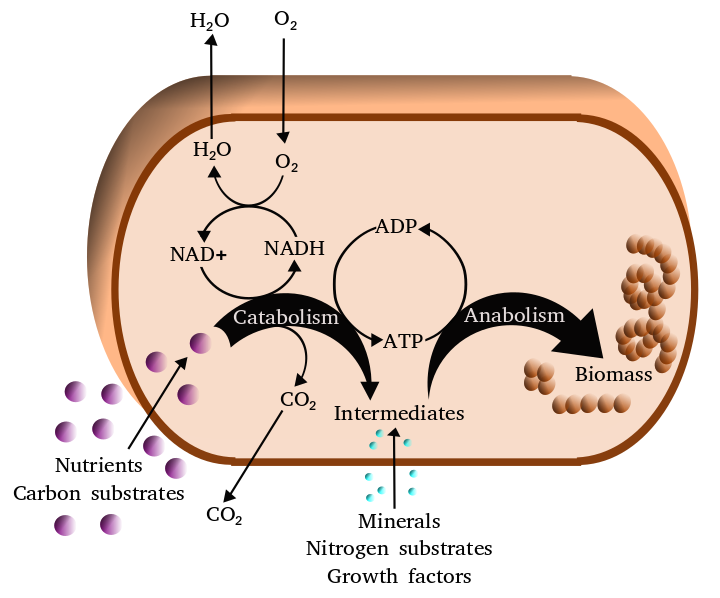
\includegraphics[width=0.7\linewidth]{./figures/bioenergetics/Metabolism} 

}

\caption{\href{https://commons.wikimedia.org/wiki/File:Metabolism.png}{Simplified view of the cellular metabolism}}\label{fig:simpleviewmet}
\end{figure}

The chemical reactions of metabolism are organized into metabolic pathways, in which one chemical is transformed through a series of steps into another chemical, each step being facilitated by a specific enzyme. Enzymes are crucial to metabolism because they allow organisms to drive desirable reactions that require energy that will not occur by themselves, by coupling them to spontaneous reactions that release energy. Enzymes act as catalysts -- they allow a reaction to proceed more rapidly -- and they also allow the regulation of the rate of a metabolic reaction, for example in response to changes in the cell's environment or to signals from other cells.

The metabolic system of a particular organism determines which substances it will find nutritious and which poisonous. For example, some prokaryotes use hydrogen sulfide as a nutrient, yet this gas is poisonous to animals. The basal metabolic rate of an organism is the measure of the amount of energy consumed by all of these chemical reactions.

A striking feature of metabolism is the similarity of the basic metabolic pathways among vastly different species. For example, the set of carboxylic acids that are best known as the intermediates in the citric acid cycle are present in all known organisms, being found in species as diverse as the unicellular bacterium Escherichia coli and huge multicellular organisms like elephants. These similarities in metabolic pathways are likely due to their early appearance in evolutionary history, and their retention because of their efficacy. The metabolism of cancer cells is also different from the metabolism of normal cells and these differences can be used to find targets for therapeutic intervention in cancer.

Most of the structures that make up animals, plants and microbes are made from four basic classes of molecule: amino acids, carbohydrates , nucleic acid and lipids (often called fats). As these molecules are vital for life, metabolic reactions either focus on making these molecules during the construction of cells and tissues, or by breaking them down and using them as a source of energy, by their digestion. These biochemicals can be joined together to make polymers such as DNA and proteins, essential macromolecules of life.

\begin{table}[!h]

\caption{\label{tab:macromol}The three essential polymeric macromolecules of life}
\centering
\begin{tabular}[t]{llll}
\toprule
Type of molecule & Name of monomer forms & Name of polymer forms & Examples of polymer forms\\
\midrule
\rowcolor{gray!6}  Amino acids & Amino acids & Proteins (made of polypeptides) & Fibrous proteins and globular proteins\\
Carbohydrates & Monosaccharides & Polysaccharides & Starch, glycogen and cellulose\\
\rowcolor{gray!6}  Nucleic acids & Nucleotides & Polynucleotides & DNA and RNA\\
\bottomrule
\end{tabular}
\end{table}

The history of the scientific study of metabolism spans several centuries and has moved from examining whole animals in early studies, to examining individual metabolic reactions in modern biochemistry. The first controlled experiments in human metabolism were published by Santorio Santorio in 1614 in his book Ars de statica medicina. He described how he weighed himself before and after eating, sleep, working, sex, fasting, drinking, and excreting. He found that most of the food he took in was lost through what he called ``insensible perspiration''.

In these early studies, the mechanisms of these metabolic processes had not been identified and a vital force was thought to animate living tissue. In the 19th century, when studying the fermentation of sugar to alcohol by yeast, \href{https://en.wikipedia.org/wiki/Louis_Pasteur}{Louis Pasteur} concluded that fermentation was catalyzed by substances within the yeast cells he called ``ferments''. He wrote that ``alcoholic fermentation is an act correlated with the life and organization of the yeast cells, not with the death or putrefaction of the cells.'' This discovery, along with the publication by Friedrich Wöhler in 1828 of a paper on the chemical synthesis of urea, and is notable for being the first organic compound prepared from wholly inorganic precursors. This proved that the organic compounds and chemical reactions found in cells were no different in principle than any other part of chemistry.

It was the discovery of enzymes at the beginning of the 20th century by \href{https://en.wikipedia.org/wiki/Eduard_Buchner}{Eduard Buchner} that separated the study of the chemical reactions of metabolism from the biological study of cells, and marked the beginnings of biochemistry. The mass of biochemical knowledge grew rapidly throughout the early 20th century. One of the most prolific of these modern biochemists was Hans Krebs who made huge contributions to the study of metabolism. He discovered the urea cycle and later, working with Hans Kornberg, the citric acid cycle and the glyoxylate cycle. Modern biochemical research has been greatly aided by the development of new techniques such as chromatography, X-ray diffraction, NMR spectroscopy, radioisotopic labelling, electron microscopy and molecular dynamics simulations. These techniques have allowed the discovery and detailed analysis of the many molecules and metabolic pathways in cells.

\hypertarget{catabolism}{%
\subsection{Catabolism}\label{catabolism}}

Catabolism is the set of metabolic processes that break down large molecules. These include breaking down and oxidizing food molecules. The purpose of the catabolic reactions is to provide the energy and components needed by anabolic reactions which build molecules. The exact nature of these catabolic reactions differ from organism to organism, and organisms can be classified based on their sources of energy and carbon (their primary nutritional groups), as shown in the table below. Organic molecules are used as a source of energy by organotrophs, while lithotrophs use inorganic substrates, and phototrophs capture sunlight as chemical energy. However, all these different forms of metabolism depend on redox reactions that involve the transfer of electrons from reduced donor molecules such as organic molecules, water, ammonia, hydrogen sulfide or ferrous ions to acceptor molecules such as oxygen, nitrate or sulfate. In animals, these reactions involve complex organic molecules that are broken down to simpler molecules, such as carbon dioxide and water. In photosynthetic organisms, such as plants and cyanobacteria, these electron-transfer reactions do not release energy but are used as a way of storing energy absorbed from sunlight.



\begin{figure}

{\centering 
\includegraphics[width=0.7\linewidth]{./figures/bioenergetics/Catabolism_schematic} 

}

\caption{\href{https://commons.wikimedia.org/wiki/File:Catabolism_schematic.svg}{Simplified diagram of catabolism of proteins, carbohydrates and fats.}}\label{fig:simplecatdia}
\end{figure}

The most common set of catabolic reactions in animals can be separated into three main stages. In the first stage, large organic molecules, such as proteins, polysaccharides or lipids, are digested into their smaller components outside cells. Next, these smaller molecules are taken up by cells and converted to smaller molecules, usually acetyl coenzyme A (acetyl-CoA), which releases some energy. Finally, the acetyl group on the CoA is oxidised to water and carbon dioxide in the citric acid cycle and electron transport chain, releasing the energy that is stored by reducing the coenzyme nicotinamide adenine dinucleotide (NAD\textsuperscript{+}) into NADH.

\hypertarget{digestion}{%
\subsection{Digestion}\label{digestion}}

Macromolecules cannot be directly processed by cells. Macromolecules must be broken into smaller units before they can be used in cell metabolism. Different classes of enzymes were being used to digest these polymers. These digestive enzymes include proteases that digest proteins into amino acids, as well as glycoside hydrolases that digest polysaccharides into simple sugars known as monosaccharides

Microbes simply secrete digestive enzymes into their surroundings, while animals only secrete these enzymes from specialized cells in their guts, including the stomach and pancreas, and salivary glands. The amino acids or sugars released by these extracellular enzymes are then pumped into cells by active transport proteins.

\hypertarget{energy-from-organic-compounds}{%
\subsection{Energy From Organic Compounds}\label{energy-from-organic-compounds}}

Carbohydrate catabolism is the breakdown of carbohydrates into smaller units. Carbohydrates are usually taken into cells once they have been digested into monosaccharides. Once inside, the major route of breakdown is glycolysis, where sugars such as glucose and fructose are converted into pyruvate and some ATP is generated. Pyruvate is an intermediate in several metabolic pathways, but the majority is converted to acetyl-CoA through aerobic (with oxygen) glycolysis and fed into the citric acid cycle. Although some more ATP is generated in the citric acid cycle, the most important product is NADH, which is made from NAD\textsuperscript{+} as the acetyl-CoA is oxidized. This oxidation releases carbon dioxide as a waste product. In anaerobic conditions, glycolysis produces lactate, through the enzyme lactate dehydrogenase re-oxidizing NADH to NAD\textsuperscript{+} for re-use in glycolysis. An alternative route for glucose breakdown is the pentose phosphate pathway, which reduces the coenzyme NADPH and produces pentose sugars such as ribose, the sugar component of nucleic acids.

Fats are catabolised by hydrolysis to free fatty acids and glycerol. The glycerol enters glycolysis and the fatty acids are broken down by beta oxidation to release acetyl-CoA, which then is fed into the citric acid cycle. Fatty acids release more energy upon oxidation than carbohydrates because carbohydrates contain more oxygen in their structures. Steroids are also broken down by some bacteria in a process similar to beta oxidation, and this breakdown process involves the release of significant amounts of acetyl-CoA, propionyl-CoA, and pyruvate, which can all be used by the cell for energy. M. tuberculosis can also grow on the lipid cholesterol as a sole source of carbon, and genes involved in the cholesterol use pathway(s) have been validated as important during various stages of the infection lifecycle of M. tuberculosis.

Amino acids are either used to synthesize proteins and other biomolecules, or oxidized to urea and carbon dioxide as a source of energy. The oxidation pathway starts with the removal of the amino group by a transaminase. The amino group is fed into the urea cycle, leaving a deaminated carbon skeleton in the form of a keto acid. Several of these keto acids are intermediates in the citric acid cycle, for example the deamination of glutamate forms α-ketoglutarate. The glucogenic amino acids can also be converted into glucose, through gluconeogenesis (discussed below).

\hypertarget{energy-transformations}{%
\section{Energy Transformations}\label{energy-transformations}}

\hypertarget{oxidative-phosphorylation}{%
\subsection{Oxidative Phosphorylation}\label{oxidative-phosphorylation}}

In oxidative phosphorylation, the electrons removed from organic molecules are transferred to oxygen and the energy released is used to make ATP. This is done in eukaryotes by a series of proteins in the membranes of mitochondria called the electron transport chain. In prokaryotes, these proteins are found in the cell's inner membrane. These proteins use the energy released from passing electrons from reduced molecules like NADH onto oxygen to pump protons across a membrane.

Pumping protons out of the mitochondria creates a proton concentration difference across the membrane and generates an electrochemical gradient. This force drives protons back into the mitochondrion through the base of an enzyme called ATP synthase. The flow of protons makes the stalk subunit rotate, causing the active site of the synthase domain to change shape and phosphorylate adenosine diphosphate -- turning it into ATP.

\hypertarget{energy-from-inorganic-compounds}{%
\subsection{Energy From Inorganic Compounds}\label{energy-from-inorganic-compounds}}

Chemolithotrophy is a type of metabolism found in prokaryotes where energy is obtained from the oxidation of inorganic compounds. These organisms can use hydrogen, reduced sulfur compounds (such as sulfide, hydrogen sulfide and thiosulfate), ferrous iron (FeII) or ammonia as sources of reducing power and they gain energy from the oxidation of these compounds with electron acceptors such as oxygen or nitrite. These microbial processes are important in global biogeochemical cycles such as acetogenesis, nitrification and denitrification and are critical for soil fertility.

\hypertarget{energy-from-light}{%
\subsection{Energy From Light}\label{energy-from-light}}

The energy in sunlight is captured by plants, cyanobacteria, purple bacteria, green sulfur bacteria and some protists. This process is often coupled to the conversion of carbon dioxide into organic compounds, as part of photosynthesis, which is discussed below. The energy capture and carbon fixation systems can however operate separately in prokaryotes, as purple bacteria and green sulfur bacteria can use sunlight as a source of energy, while switching between carbon fixation and the fermentation of organic compounds.

In many organisms, the capture of solar energy is similar in principle to oxidative phosphorylation, as it involves the storage of energy as a proton concentration gradient. This proton motive force then drives ATP synthesis The electrons needed to drive this electron transport chain come from light-gathering proteins called photosynthetic reaction centres. Reaction centers are classed into two types depending on the nature of photosynthetic pigment present, with most photosynthetic bacteria only having one type, while plants and cyanobacteria have two.

In plants, algae, and cyanobacteria, photosystem II uses light energy to remove electrons from water, releasing oxygen as a waste product. The electrons then flow to the cytochrome b6f complex, which uses their energy to pump protons across the thylakoid membrane in the chloroplast. These protons move back through the membrane as they drive the ATP synthase, as before. The electrons then flow through photosystem I and can then either be used to reduce the coenzyme NADP\textsuperscript{+}.fThese cooenzyme can be used in the Calvin cycle, which is discussed below, or recycled for further ATP generation.

\hypertarget{anabolism}{%
\subsection{Anabolism}\label{anabolism}}

Anabolism is the set of constructive metabolic processes where the energy released by catabolism is used to synthesize complex molecules. In general, the complex molecules that make up cellular structures are constructed step-by-step from small and simple precursors. Anabolism involves three basic stages. First, the production of precursors such as amino acids, monosaccharides, isoprenoids and nucleotides, secondly, their activation into reactive forms using energy from ATP, and thirdly, the assembly of these precursors into complex molecules such as proteins, polysaccharides, lipids and nucleic acids.

Anabolism in organisms can be different according to the source of constructed molecules in their cells. Autotrophs such as plants can construct the complex organic molecules in cells such as polysaccharides and proteins from simple molecules like carbon dioxide and water. Heterotrophs, on the other hand, require a source of more complex substances, such as monosaccharides and amino acids, to produce these complex molecules. Organisms can be further classified by ultimate source of their energy: photoautotrophs and photoheterotrophs obtain energy from light, whereas chemoautotrophs and chemoheterotrophs obtain energy from inorganic oxidation reactions.

\hypertarget{carbon-fixation}{%
\subsection{Carbon Fixation}\label{carbon-fixation}}

Photosynthesis is the synthesis of carbohydrates from sunlight and carbon dioxide (CO\textsubscript{2}). In plants, cyanobacteria and algae, oxygenic photosynthesis splits water, with oxygen produced as a waste product. This process uses the ATP and NADPH produced by the photosynthetic reaction centres, as described above, to convert CO\textsubscript{2} into glycerate 3-phosphate, which can then be converted into glucose. This carbon-fixation reaction is carried out by the enzyme RuBisCO as part of the Calvin cycle. Three types of photosynthesis occur in plants, C3 carbon fixation, C4 carbon fixation and CAM photosynthesis. These differ by the route that carbon dioxide takes to the Calvin cycle, with C3 plants fixing CO\textsubscript{2} directly, while C4 and CAM photosynthesis incorporate the CO\textsubscript{2} into other compounds first, as adaptations to deal with intense sunlight and dry conditions.

In photosynthetic prokaryotes the mechanisms of carbon fixation are more diverse. Here, carbon dioxide can be fixed by the Calvin cycle, a reversed citric acid cycle, or the carboxylation of acetyl-CoA. Prokaryotic chemoautotrophs also fix CO\textsubscript{2} through the Calvin cycle, but use energy from inorganic compounds to drive the reaction.

\hypertarget{carbohydrates-and-glycans}{%
\subsection{Carbohydrates And Glycans}\label{carbohydrates-and-glycans}}

In carbohydrate anabolism, simple organic acids can be converted into monosaccharides such as glucose and then used to assemble polysaccharides such as starch. The generation of glucose from compounds like pyruvate, lactate, glycerol, glycerate 3-phosphate and amino acids is called gluconeogenesis. Gluconeogenesis converts pyruvate to glucose-6-phosphate through a series of intermediates, many of which are shared with glycolysis. However, this pathway is not simply glycolysis run in reverse, as several steps are catalyzed by non-glycolytic enzymes. This is important as it allows the formation and breakdown of glucose to be regulated separately, and prevents both pathways from running simultaneously in a futile cycle.

Although fat is a common way of storing energy, in vertebrates such as humans the fatty acids in these stores cannot be converted to glucose through gluconeogenesis as these organisms cannot convert acetyl-CoA into pyruvate; plants do, but animals do not, have the necessary enzymatic machinery. As a result, after long-term starvation, vertebrates need to produce ketone bodies from fatty acids to replace glucose in tissues such as the brain that cannot metabolize fatty acids. In other organisms such as plants and bacteria, this metabolic problem is solved using the glyoxylate cycle, which bypasses the decarboxylation step in the citric acid cycle and allows the transformation of acetyl-CoA to oxaloacetate, where it can be used for the production of glucose. Other than fat, glucose is stored in most tissues, as an energy resource available within the tissue through glycogenesis which was usually being used to maintained glucose level in blood.

Polysaccharides and glycans are made by the sequential addition of monosaccharides by glycosyltransferase from a reactive sugar-phosphate donor such as uridine diphosphate glucose (UDP-Glc) to an acceptor hydroxyl group on the growing polysaccharide. As any of the hydroxyl groups on the ring of the substrate can be acceptors, the polysaccharides produced can have straight or branched structures. The polysaccharides produced can have structural or metabolic functions themselves, or be transferred to lipids and proteins by enzymes called oligosaccharyltransferases.

\hypertarget{fatty-acids-isoprenoids-and-sterol}{%
\subsection{Fatty Acids, Isoprenoids and Sterol}\label{fatty-acids-isoprenoids-and-sterol}}

Simplified version of the steroid synthesis pathway with the intermediates isopentenyl pyrophosphate (IPP), dimethylallyl pyrophosphate , geranyl pyrophosphate (GPP) and squalene shown. Some intermediates are omitted for clarity.
Fatty acids are made by fatty acid synthases that polymerize and then reduce acetyl-CoA units. The acyl chains in the fatty acids are extended by a cycle of reactions that add the acyl group, reduce it to an alcohol, dehydrate it to an alkene group and then reduce it again to an alkane group. The enzymes of fatty acid biosynthesis are divided into two groups: in animals and fungi, all these fatty acid synthase reactions are carried out by a single multifunctional type I protein, while in plant plastids and bacteria separate type II enzymes perform each step in the pathway.

Terpenes and isoprenoids are a large class of lipids that include the carotenoids and form the largest class of plant natural products. These compounds are made by the assembly and modification of isoprene units donated from the reactive precursors isopentenyl pyrophosphate and dimethylallyl pyrophosphate. These precursors can be made in different ways. In animals and archaea, the mevalonate pathway produces these compounds from acetyl-CoA, while in plants and bacteria the non-mevalonate pathway uses pyruvate and glyceraldehyde 3-phosphate as substrates. One important reaction that uses these activated isoprene donors is sterol biosynthesis. Here, the isoprene units are joined together to make squalene and then folded up and formed into a set of rings to make lanosterol. Lanosterol can then be converted into other sterol such as cholesterol and ergosterol.

\hypertarget{proteins-1}{%
\subsection{Proteins}\label{proteins-1}}

Organisms vary in their ability to synthesize the 20 common amino acids. Most bacteria and plants can synthesize all twenty, but mammals can only synthesize eleven nonessential amino acids, so nine essential amino acids must be obtained from food. Some simple parasites, such as the bacteria Mycoplasma pneumoniae, lack all amino acid synthesis and take their amino acids directly from their hosts. All amino acids are synthesized from intermediates in glycolysis, the citric acid cycle, or the pentose phosphate pathway. Nitrogen is provided by glutamate and glutamine. Nonessensial amino acid synthesis depends on the formation of the appropriate alpha-keto acid, which is then transaminated to form an amino acid.

Amino acids are made into proteins by being joined together in a chain of peptide bonds. Each different protein has a unique sequence of amino acid residues: this is its primary structure. Just as the letters of the alphabet can be combined to form an almost endless variety of words, amino acids can be linked in varying sequences to form a huge variety of proteins. Proteins are made from amino acids that have been activated by attachment to a transfer RNA molecule through an ester bond. This aminoacyl-tRNA precursor is produced in an ATP-dependent reaction carried out by an aminoacyl tRNA synthetase. This aminoacyl-tRNA is then a substrate for the ribosome, which joins the amino acid onto the elongating protein chain, using the sequence information in a messenger RNA.

\hypertarget{nucleotide-synthesis-and-salvage}{%
\subsection{Nucleotide Synthesis And Salvage}\label{nucleotide-synthesis-and-salvage}}

Nucleotides are made from amino acids, carbon dioxide and formic acid in pathways that require large amounts of metabolic energy. Consequently, most organisms have efficient systems to salvage preformed nucleotides. Purines are synthesized as nucleosides (bases attached to ribose). Both adenine and guanine are made from the precursor nucleoside inosine monophosphate, which is synthesized using atoms from the amino acids glycine, glutamine, and aspartic acid, as well as formate transferred from the coenzyme tetrahydrofolate. Pyrimidines, on the other hand, are synthesized from the base orotate, which is formed from glutamine and aspartate.

\hypertarget{enzymes}{%
\section{Enzymes}\label{enzymes}}

Enzymes are proteins that act as biological catalysts (biocatalysts). Catalysts accelerate chemical reactions. A catalyst increases the rate of reaction without being consumed in the reaction. In addition, the catalyst lowers the activation energy, but it does not change the energies of the original reactants or products, and so does not change equilibrium. Rather, the reactant energy and the product energy remain the same and only the activation energy is altered (lowered). A catalyst is able to reduce the activation energy by forming a transition state in a more favorable manner. Catalysts, by nature, create a more ``comfortable'' fit for the substrate of a reaction to progress to a transition state. This is possible due to a release of energy that occurs when the substrate binds to the active site of a catalyst. This energy is known as Binding Energy. Upon binding to a catalyst, substrates partake in numerous stabilizing forces while within the active site (i.e.~Hydrogen bonding, van der Waals forces). Specific and favorable bonding occurs within the active site until the substrate forms to become the high-energy transition state. Forming the transition state is more favorable with the catalyst because the favorable stabilizing interactions within the active site release energy. A chemical reaction is able to manufacture a high-energy transition state molecule more readily when there is a stabilizing fit within the active site of a catalyst. The binding energy of a reaction is this energy released when favorable interactions between substrate and catalyst occur. The binding energy released assists in achieving the unstable transition state. Reactions otherwise without catalysts need a higher input of energy to achieve the transition state. Non-catalyzed reactions do not have free energy available from active site stabilizing interactions, such as catalytic enzyme reactions.

Enzymes are known to catalyze more than 5,000 biochemical reaction types. Other biocatalysts are catalytic RNA molecules, called ribozymes. Enzymes' specificity comes from their unique three-dimensional structures.

The molecules upon which enzymes may act are called substrates, and the enzyme converts the substrates into different molecules known as products. Almost all metabolic processes in the cell need enzyme catalysis in order to occur at rates fast enough to sustain life. Metabolic pathways depend upon enzymes to catalyze individual steps.

Like all catalysts, enzymes increase the reaction rate by lowering its activation energy. Some enzymes can make their conversion of substrate to product occur many millions of times faster. An extreme example is orotidine 5'-phosphate decarboxylase, which allows a reaction that would otherwise take millions of years to occur in milliseconds. Chemically, enzymes are like any catalyst and are not consumed in chemical reactions, nor do they alter the equilibrium of a reaction. Enzymes differ from most other catalysts by being much more specific. Enzyme activity can be affected by other molecules: inhibitors are molecules that decrease enzyme activity, and activators are molecules that increase activity. Many therapeutic drugs and poisons are enzyme inhibitors. An enzyme's activity decreases markedly outside its optimal temperature and pH, and many enzymes are (permanently) denatured when exposed to excessive heat, losing their structure and catalytic properties.



\begin{figure}

{\centering 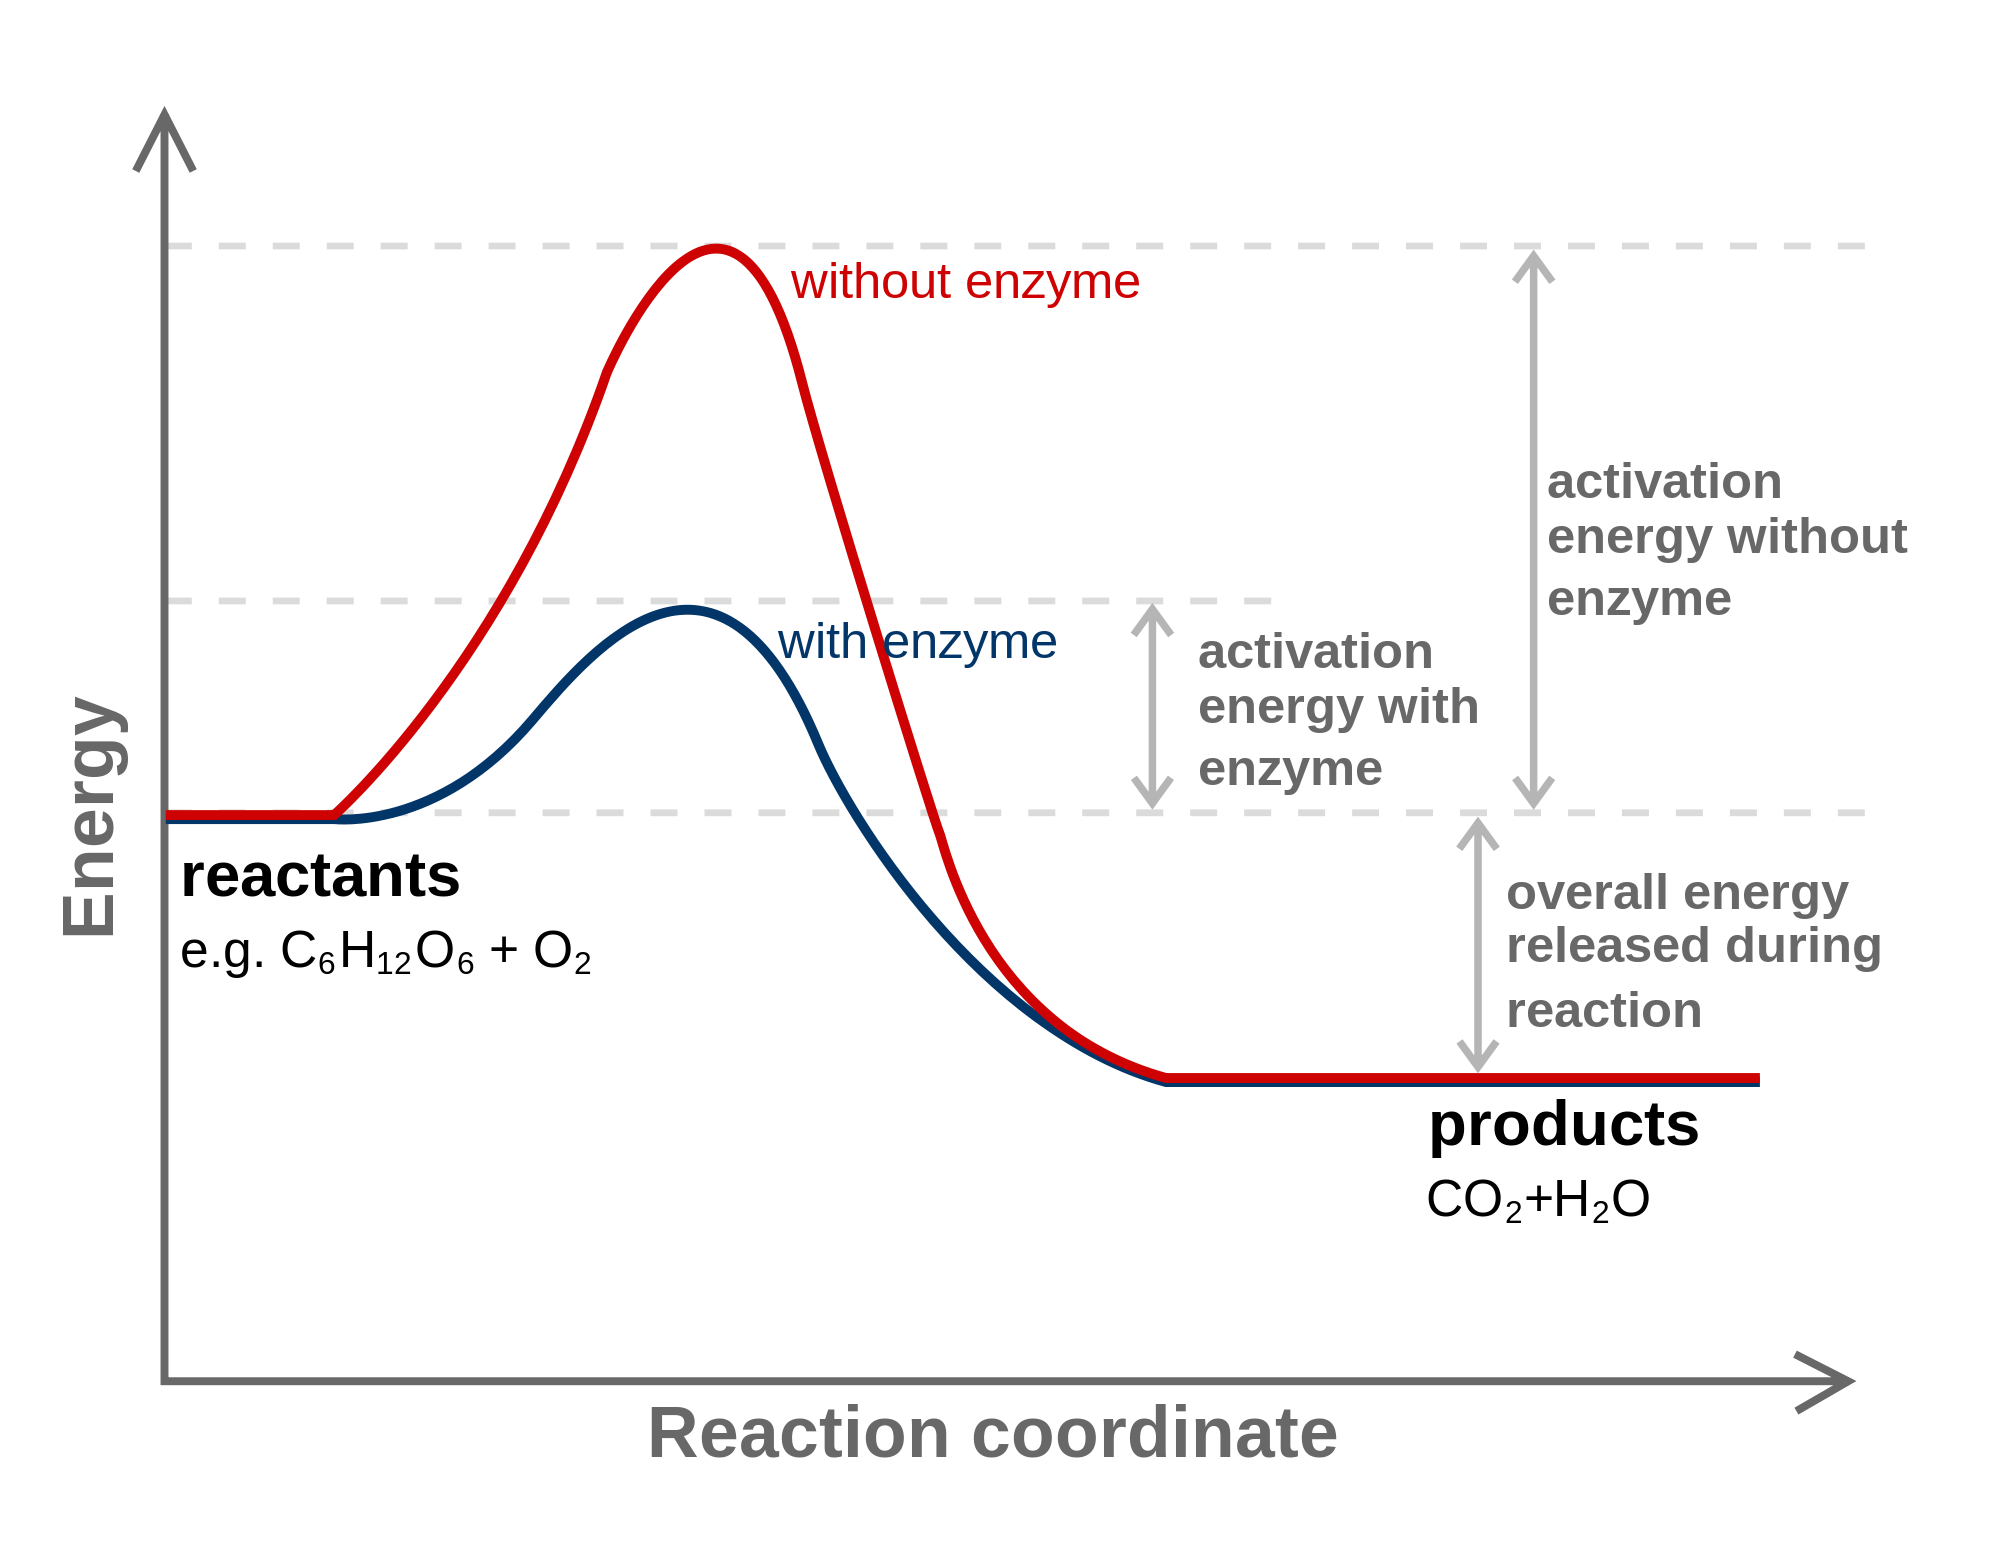
\includegraphics[width=0.7\linewidth]{./figures/bioenergetics/Activation2_updated} 

}

\caption{\href{https://commons.wikimedia.org/wiki/File:Activation2_updated.svg}{Example of an enzyme-catalysed exothermic reaction}}\label{fig:activationenergy}
\end{figure}

Some enzymes are used commercially, for example, in the synthesis of antibiotics. Some household products use enzymes to speed up chemical reactions: enzymes in biological washing powders break down protein, starch or fat stains on clothes, and enzymes in meat tenderizer break down proteins into smaller molecules, making the meat easier to chew.

By the late 17th and early 18th centuries, the digestion of meat by stomach secretions and the conversion of starch to sugars by plant extracts and saliva were known but the mechanisms by which these occurred had not been identified.

French chemist \href{https://en.wikipedia.org/wiki/Anselme_Payen}{Anselme Payen} was the first to discover an enzyme, diastase, in 1833. A few decades later, when studying the fermentation of sugar to alcohol by yeast, Louis Pasteur concluded that this fermentation was caused by a vital force contained within the yeast cells called ``ferments'', which were thought to function only within living organisms. He wrote that ``alcoholic fermentation is an act correlated with the life and organization of the yeast cells, not with the death or putrefaction of the cells.''

Eduard Buchner submitted his first paper on the study of yeast extracts in 1897. In a series of experiments at the University of Berlin, he found that sugar was fermented by yeast extracts even when there were no living yeast cells in the mixture. He named the enzyme that brought about the fermentation of sucrose ``zymase''. In 1907, he received the Nobel Prize in Chemistry for ``his discovery of cell-free fermentation''. Following Buchner's example, enzymes are usually named according to the reaction they carry out: the suffix -ase is combined with the name of the substrate (e.g., lactase is the enzyme that cleaves lactose) or to the type of reaction (e.g., DNA polymerase forms DNA polymers).

The biochemical identity of enzymes was still unknown in the early 1900s. Many scientists observed that enzymatic activity was associated with proteins, but others (such as Nobel laureate \href{https://en.wikipedia.org/wiki/Richard_Willstätter}{Richard Willstätter}) argued that proteins were merely carriers for the true enzymes and that proteins per se were incapable of catalysis. In 1926, \href{https://en.wikipedia.org/wiki/James_B._Sumner}{James B. Sumner} showed that the enzyme urease was a pure protein and crystallized it; he did likewise for the enzyme catalase in 1937. The conclusion that pure proteins can be enzymes was definitively demonstrated by \href{https://en.wikipedia.org/wiki/John_Howard_Northrop}{John Howard Northrop} and \href{https://en.wikipedia.org/wiki/Wendell_Meredith_Stanley}{Wendell Meredith Stanley}, who worked on the digestive enzymes pepsin (1930), trypsin and chymotrypsin. These three scientists were awarded the 1946 Nobel Prize in Chemistry.

The discovery that enzymes could be crystallized eventually allowed their structures to be solved by x-ray crystallography. This was first done for lysozyme, an enzyme found in tears, saliva and egg whites that digests the coating of some bacteria; the structure was solved by a group led by \href{https://en.wikipedia.org/wiki/David_Chilton_Phillips}{David Chilton Phillips} and published in 1965. This high-resolution structure of lysozyme marked the beginning of the field of structural biology and the effort to understand how enzymes work at an atomic level of detail.

An enzyme's name is often derived from its substrate or the chemical reaction it catalyzes, with the word ending in -ase. Examples are lactase, alcohol dehydrogenase and DNA polymerase. Different enzymes that catalyze the same chemical reaction are called isozymes.

Enzymes are generally globular proteins, acting alone or in larger complexes. The sequence of the amino acids specifies the structure which in turn determines the catalytic activity of the enzyme. Although structure determines function, a novel enzymatic activity cannot yet be predicted from structure alone. Enzyme structures unfold (denature) when heated or exposed to chemical denaturants and this disruption to the structure typically causes a loss of activity. Enzyme denaturation is normally linked to temperatures above a species' normal level; as a result, enzymes from bacteria living in volcanic environments such as hot springs are prized by industrial users for their ability to function at high temperatures, allowing enzyme-catalysed reactions to be operated at a very high rate.

Enzymes are usually much larger than their substrates. Sizes range from just 62 amino acid residues, for the monomer of 4-oxalocrotonate tautomerase, to over 2,500 residues in the animal fatty acid synthase. Only a small portion of their structure (around 2--4 amino acids) is directly involved in catalysis: the catalytic site. This catalytic site is located next to one or more binding sites where residues orient the substrates. The catalytic site and binding site together compose the enzyme's active site. The remaining majority of the enzyme structure serves to maintain the precise orientation and dynamics of the active site.

In some enzymes, no amino acids are directly involved in catalysis; instead, the enzyme contains sites to bind and orient catalytic cofactors. Enzyme structures may also contain allosteric sites where the binding of a small molecule causes a conformational change that increases or decreases activity.

A small number of RNA-based biological catalysts called ribozymes exist, which again can act alone or in complex with proteins. The most common of these is the ribosome which is a complex of protein and catalytic RNA components.

Enzymes must bind their substrates before they can catalyse any chemical reaction. Enzymes are usually very specific as to what substrates they bind and then the chemical reaction catalysed. Specificity is achieved by binding pockets with complementary shape, charge and hydrophilic/hydrophobic characteristics to the substrates. Enzymes can therefore distinguish between very similar substrate molecules to be chemoselective, regioselective and stereospecific.

Some of the enzymes showing the highest specificity and accuracy are involved in the copying and expression of the genome. Some of these enzymes have ``proof-reading'' mechanisms. Here, an enzyme such as DNA polymerase catalyzes a reaction in a first step and then checks that the product is correct in a second step. This two-step process results in average error rates of less than 1 error in 100 million reactions in high-fidelity mammalian polymerases. Similar proofreading mechanisms are also found in RNA polymerase, aminoacyl tRNA synthetases and ribosomes.

Conversely, some enzymes display enzyme promiscuity, having broad specificity and acting on a range of different physiologically relevant substrates. Many enzymes possess small side activities which arose fortuitously (i.e.~neutrally), which may be the starting point for the evolutionary selection of a new function.

To explain the observed specificity of enzymes, in 1894 \href{https://en.wikipedia.org/wiki/Emil_Fischer}{Emil Fischer} proposed that both the enzyme and the substrate possess specific complementary geometric shapes that fit exactly into one another. This is often referred to as ``the lock and key'' model. This early model explains enzyme specificity, but fails to explain the stabilization of the transition state that enzymes achieve.

In 1958, \href{https://en.wikipedia.org/wiki/Daniel_E._Koshland_Jr.}{Daniel Koshland} suggested a modification to the lock and key model: since enzymes are rather flexible structures, the active site is continuously reshaped by interactions with the substrate as the substrate interacts with the enzyme. As a result, the substrate does not simply bind to a rigid active site; the amino acid side-chains that make up the active site are molded into the precise positions that enable the enzyme to perform its catalytic function. In some cases, such as glycosidases, the substrate molecule also changes shape slightly as it enters the active site. The active site continues to change until the substrate is completely bound, at which point the final shape and charge distribution is determined. Induced fit may enhance the fidelity of molecular recognition in the presence of competition and noise via the conformational proofreading mechanism.

Enzymes can accelerate reactions in several ways, all of which lower the activation energy (ΔG, Gibbs free energy)

\begin{itemize}
\tightlist
\item
  By stabilizing the transition state:
\item
  Creating an environment with a charge distribution complementary to that of the transition state to lower its energy
\item
  By providing an alternative reaction pathway:
\item
  Temporarily reacting with the substrate, forming a covalent intermediate to provide a lower energy transition state
\item
  By destabilising the substrate ground state:
\item
  Distorting bound substrate(s) into their transition state form to reduce the energy required to reach the transition state
\item
  By orienting the substrates into a productive arrangement to reduce the reaction entropy change (the contribution of this mechanism to catalysis is relatively small)
\end{itemize}

Enzymes may use several of these mechanisms simultaneously. For example, proteases such as trypsin perform covalent catalysis using a catalytic triad, stabilise charge build-up on the transition states using an oxyanion hole, complete hydrolysis using an oriented water substrate.

Enzymes are not rigid, static structures; instead they have complex internal dynamic motions -- that is, movements of parts of the enzyme's structure such as individual amino acid residues, groups of residues forming a protein loop or unit of secondary structure, or even an entire protein domain. These motions give rise to a conformational ensemble of slightly different structures that interconvert with one another at equilibrium. Different states within this ensemble may be associated with different aspects of an enzyme's function. For example, different conformations of the enzyme dihydrofolate reductase are associated with the substrate binding, catalysis, cofactor release, and product release steps of the catalytic cycle, consistent with catalytic resonance theory.

Substrate presentation is a process where the enzyme is sequestered away from its substrate. Enzymes can be sequestered to the plasma membrane away from a substrate in the nucleus or cytosol. Or within the membrane, an enzyme can be sequestered into lipid rafts away from its substrate in the disordered region. When the enzyme is releases it mixes with its substrate. Alternatively, the enzyme can be sequestered near its substrate to activate the enzyme. For example, the enzyme can be soluble and upon activation bind to a lipid in the plasma membrane and then act upon molecules in the plasma membrane.

\hypertarget{allosteric-modulation}{%
\subsection{Allosteric Modulation}\label{allosteric-modulation}}

Allosteric sites are pockets on the enzyme, distinct from the active site, that bind to molecules in the cellular environment. These molecules then cause a change in the conformation or dynamics of the enzyme that is transduced to the active site and thus affects the reaction rate of the enzyme. In this way, allosteric interactions can either inhibit or activate enzymes. Allosteric interactions with metabolites upstream or downstream in an enzyme's metabolic pathway cause feedback regulation, altering the activity of the enzyme according to the flux through the rest of the pathway.

\hypertarget{cofactors-of-enzymes-and-coenzymes}{%
\subsection{Cofactors of Enzymes and Coenzymes}\label{cofactors-of-enzymes-and-coenzymes}}

Some enzymes do not need additional components to show full activity. Others require non-protein molecules called cofactors to be bound for activity. Cofactors can be either inorganic (e.g., metal ions and iron-sulfur clusters) or organic compounds (e.g., flavin and heme). These cofactors serve many purposes; for instance, metal ions can help in stabilizing nucleophilic species within the active site. Organic cofactors can be either coenzymes, which are released from the enzyme's active site during the reaction, or prosthetic groups, which are tightly bound to an enzyme. Organic prosthetic groups can be covalently bound (e.g., biotin in enzymes such as pyruvate carboxylase).

An example of an enzyme that contains a cofactor is carbonic anhydrase, which uses a zinc cofactor bound as part of its active site. These tightly bound ions or molecules are usually found in the active site and are involved in catalysis. For example, flavin and heme cofactors are often involved in redox reactions.

Enzymes that require a cofactor but do not have one bound are called apoenzymes or apoproteins. An enzyme together with the cofactor(s) required for activity is called a holoenzyme (or haloenzyme). The term holoenzyme can also be applied to enzymes that contain multiple protein subunits, such as the DNA polymerases; here the holoenzyme is the complete complex containing all the subunits needed for activity.

Coenzymes are small organic molecules that can be loosely or tightly bound to an enzyme. Coenzymes transport chemical groups from one enzyme to another. Examples include NADH, NADPH and adenosine triphosphate (ATP). Some coenzymes, such as flavin mononucleotide (FMN), flavin adenine dinucleotide (FAD), thiamine pyrophosphate (TPP), and tetrahydrofolate (THF), are derived from vitamins. These coenzymes cannot be synthesized by the body de novo and closely related compounds (vitamins) must be acquired from the diet. The chemical groups carried include:

\begin{itemize}
\tightlist
\item
  the hydride ion (H\textsuperscript{-}), carried by NAD or NADP\textsuperscript{+}
\item
  the phosphate group, carried by adenosine triphosphate
\item
  the acetyl group, carried by coenzyme A
\item
  formyl, methenyl or methyl groups, carried by folic acid and
\item
  the methyl group, carried by S-adenosylmethionine
\end{itemize}

Since coenzymes are chemically changed as a consequence of enzyme action, it is useful to consider coenzymes to be a special class of substrates, or second substrates, which are common to many different enzymes. For example, about 1000 enzymes are known to use the coenzyme NADH.

Coenzymes are usually continuously regenerated and their concentrations maintained at a steady level inside the cell. For example, NADPH is regenerated through the pentose phosphate pathway and S-adenosylmethionine by methionine adenosyltransferase. This continuous regeneration means that small amounts of coenzymes can be used very intensively. For example, the human body turns over its own weight in ATP each day.

\hypertarget{inhibition-of-enzymes}{%
\subsection{Inhibition of Enzymes}\label{inhibition-of-enzymes}}

An enzyme binding site that would normally bind substrate can alternatively bind a competitive inhibitor, preventing substrate access. Dihydrofolate reductase is inhibited by methotrexate which prevents binding of its substrate, folic acid. Binding site in blue, inhibitor in green, and substrate in black. (PDB: 4QI9​)
Two dimensional representations of the chemical structure of folic acid and methotrexate highlighting the differences between these two substances (amidation of pyrimidone and methylation of secondary amine).
The coenzyme folic acid (left) and the anti-cancer drug methotrexate (right) are very similar in structure (differences show in green). As a result, methotrexate is a competitive inhibitor of many enzymes that use folates.
Main article: Enzyme inhibitor
Enzyme reaction rates can be decreased by various types of enzyme inhibitors.

A competitive inhibitor and substrate cannot bind to the enzyme at the same time. Often competitive inhibitors strongly resemble the real substrate of the enzyme. For example, the drug methotrexate is a competitive inhibitor of the enzyme dihydrofolate reductase, which catalyzes the reduction of dihydrofolate to tetrahydrofolate. The similarity between the structures of dihydrofolate and this drug are shown in the accompanying figure. This type of inhibition can be overcome with high substrate concentration. In some cases, the inhibitor can bind to a site other than the binding-site of the usual substrate and exert an allosteric effect to change the shape of the usual binding-site.

A non-competitive inhibitor binds to a site other than where the substrate binds. The substrate still binds with its usual affinity and hence Km remains the same. However the inhibitor reduces the catalytic efficiency of the enzyme so that Vmax is reduced. In contrast to competitive inhibition, non-competitive inhibition cannot be overcome with high substrate concentration.

An uncompetitive inhibitor cannot bind to the free enzyme, only to the enzyme-substrate complex; hence, these types of inhibitors are most effective at high substrate concentration. In the presence of the inhibitor, the enzyme-substrate complex is inactive. This type of inhibition is rare.

A mixed inhibitor binds to an allosteric site and the binding of the substrate and the inhibitor affect each other. The enzyme's function is reduced but not eliminated when bound to the inhibitor. This type of inhibitor does not follow the Michaelis--Menten equation.

An irreversible inhibitor permanently inactivates the enzyme, usually by forming a covalent bond to the protein. Penicillin and aspirin are common drugs that act in this manner.

In many organisms, inhibitors may act as part of a feedback mechanism. If an enzyme produces too much of one substance in the organism, that substance may act as an inhibitor for the enzyme at the beginning of the pathway that produces it, causing production of the substance to slow down or stop when there is sufficient amount. This is a form of negative feedback. Major metabolic pathways such as the citric acid cycle make use of this mechanism.

Since inhibitors modulate the function of enzymes they are often used as drugs. Many such drugs are reversible competitive inhibitors that resemble the enzyme's native substrate, similar to methotrexate above; other well-known examples include statins used to treat high cholesterol, and protease inhibitors used to treat retroviral infections such as HIV. A common example of an irreversible inhibitor that is used as a drug is aspirin, which inhibits the COX-1 and COX-2 enzymes that produce the inflammation messenger prostaglandin. Other enzyme inhibitors are poisons. For example, the poison cyanide is an irreversible enzyme inhibitor that combines with the copper and iron in the active site of the enzyme cytochrome c oxidase and blocks cellular respiration.

\hypertarget{factors-affecting-enzyme-activity}{%
\subsection{Factors Affecting Enzyme Activity}\label{factors-affecting-enzyme-activity}}

As enzymes are made up of proteins, their actions are sensitive to change in many physio chemical factors such as pH, temperature, substrate concentration, etc.

Enzymes serve a wide variety of functions inside living organisms. They are indispensable for signal transduction and cell regulation, often via kinases and phosphatases. They also generate movement, with myosin hydrolyzing ATP to generate muscle contraction, and also transport cargo around the cell as part of the cytoskeleton. Other ATPases in the cell membrane are ion pumps involved in active transport. Enzymes are also involved in more exotic functions, such as luciferase generating light in fireflies. Viruses can also contain enzymes for infecting cells, such as the HIV integrase and reverse transcriptase, or for viral release from cells, like the influenza virus neuraminidase.

An important function of enzymes is in the digestive systems of animals. Enzymes such as amylases and proteases break down large molecules (starch or proteins, respectively) into smaller ones, so they can be absorbed by the intestines. Starch molecules, for example, are too large to be absorbed from the intestine, but enzymes hydrolyze the starch chains into smaller molecules such as maltose and eventually glucose, which can then be absorbed. Different enzymes digest different food substances. In ruminants, which have herbivorous diets, microorganisms in the gut produce another enzyme, cellulase, to break down the cellulose cell walls of plant fiber.

Several enzymes can work together in a specific order, creating metabolic pathways. In a metabolic pathway, one enzyme takes the product of another enzyme as a substrate. After the catalytic reaction, the product is then passed on to another enzyme. Sometimes more than one enzyme can catalyze the same reaction in parallel; this can allow more complex regulation with, for example, a low constant activity provided by one enzyme but an inducible high activity from a second enzyme.

Enzymes determine what steps occur in these pathways. Without enzymes, metabolism would neither progress through the same steps and could not be regulated to serve the needs of the cell. Most central metabolic pathways are regulated at a few key steps, typically through enzymes whose activity involves the hydrolysis of ATP. Because this reaction releases so much energy, other reactions that are thermodynamically unfavorable can be coupled to ATP hydrolysis, driving the overall series of linked metabolic reactions.

\hypertarget{control-of-activity}{%
\subsection{Control of activity}\label{control-of-activity}}

There are five main ways that enzyme activity is controlled in the cell.

Enzymes can be either activated or inhibited by other molecules. For example, the end product(s) of a metabolic pathway are often inhibitors for one of the first enzymes of the pathway (usually the first irreversible step, called committed step), thus regulating the amount of end product made by the pathways. Such a regulatory mechanism is called a negative feedback mechanism, because the amount of the end product produced is regulated by its own concentration. Negative feedback mechanism can effectively adjust the rate of synthesis of intermediate metabolites according to the demands of the cells. This helps with effective allocations of materials and energy economy, and it prevents the excess manufacture of end products. Like other homeostatic devices, the control of enzymatic action helps to maintain a stable internal environment in living organisms.

\hypertarget{post-translational-modification}{%
\subsection{Post-translational Modification}\label{post-translational-modification}}

Examples of post-translational modification include phosphorylation, myristoylation and glycosylation. For example, in the response to insulin, the phosphorylation of multiple enzymes, including glycogen synthase, helps control the synthesis or degradation of glycogen and allows the cell to respond to changes in blood sugar. Another example of post-translational modification is the cleavage of the polypeptide chain. Chymotrypsin, a digestive protease, is produced in inactive form as chymotrypsinogen in the pancreas and transported in this form to the stomach where it is activated. This stops the enzyme from digesting the pancreas or other tissues before it enters the gut. This type of inactive precursor to an enzyme is known as a zymogen or proenzyme.

\hypertarget{quantity}{%
\subsection{Quantity}\label{quantity}}

Enzyme production (transcription and translation of enzyme genes) can be enhanced or diminished by a cell in response to changes in the cell's environment. This form of gene regulation is called enzyme induction. For example, bacteria may become resistant to antibiotics such as penicillin because enzymes called beta-lactamases are induced that hydrolyse the crucial beta-lactam ring within the penicillin molecule. Another example comes from enzymes in the liver called cytochrome P450 oxidases, which are important in drug metabolism. Induction or inhibition of these enzymes can cause drug interactions. Enzyme levels can also be regulated by changing the rate of enzyme degradation. The opposite of enzyme induction is enzyme repression.

\hypertarget{subcellular-distribution}{%
\subsection{Subcellular Distribution}\label{subcellular-distribution}}

Enzymes can be compartmentalized, with different metabolic pathways occurring in different cellular compartments. For example, fatty acids are synthesized by one set of enzymes in the cytosol, endoplasmic reticulum and Golgi and used by a different set of enzymes as a source of energy in the mitochondrion, through β-oxidation. In addition, trafficking of the enzyme to different compartments may change the degree of protonation (e.g., the neutral cytoplasm and the acidic lysosome) or oxidative state (e.g., oxidizing periplasm or reducing cytoplasm) which in turn affects enzyme activity. In contrast to partitioning into membrane bound organelles, enzyme subcellular localisation may also be altered through polymerisation of enzymes into macromolecular cytoplasmic filaments.

\hypertarget{organ-specialization}{%
\subsection{Organ Specialization}\label{organ-specialization}}

In multicellular eukaryotes, cells in different organs and tissues have different patterns of gene expression and therefore have different sets of enzymes (known as isozymes) available for metabolic reactions. This provides a mechanism for regulating the overall metabolism of the organism. For example, hexokinase, the first enzyme in the glycolysis pathway, has a specialized form called glucokinase expressed in the liver and pancreas that has a lower affinity for glucose yet is more sensitive to glucose concentration. This enzyme is involved in sensing blood sugar and regulating insulin production.

\hypertarget{coenzymes}{%
\subsection{Coenzymes}\label{coenzymes}}

Metabolism involves a vast array of chemical reactions, but most fall under a few basic types of reactions that involve the transfer of functional groups of atoms and their bonds within molecules. This common chemistry allows cells to use a small set of metabolic intermediates to carry chemical groups between different reactions. These group-transfer intermediates are called coenzymes. Each class of group-transfer reactions is carried out by a particular coenzyme, which is the substrate for a set of enzymes that produce it, and a set of enzymes that consume it. These coenzymes are therefore continuously made, consumed and then recycled.

One central coenzyme is adenosine triphosphate (ATP), the universal energy currency of cells. This nucleotide is used to transfer chemical energy between different chemical reactions. There is only a small amount of ATP in cells, but as it is continuously regenerated, the human body can use about its own weight in ATP per day. ATP acts as a bridge between catabolism and anabolism. Catabolism breaks down molecules, and anabolism puts them together. Catabolic reactions generate ATP, and anabolic reactions consume it. It also serves as a carrier of phosphate groups in phosphorylation reactions.

A vitamin is an organic compound needed in small quantities that cannot be made in cells. In human nutrition, most vitamins function as coenzymes after modification; for example, all water-soluble vitamins are phosphorylated or are coupled to nucleotides when they are used in cells. Nicotinamide adenine dinucleotide (NAD\textsuperscript{+}), a derivative of vitamin B3 (niacin), is an important coenzyme that acts as a hydrogen acceptor. Hundreds of separate types of dehydrogenases remove electrons from their substrates and reduce NAD\textsuperscript{+} into NADH. This reduced form of the coenzyme is then a substrate for any of the reductases in the cell that need to reduce their substrates. Nicotinamide adenine dinucleotide exists in two related forms in the cell, NADH and NADPH. The NAD\textsuperscript{+}/NADH form is more important in catabolic reactions, while NADP\textsuperscript{+}/NADPH is used in anabolic reactions.

\hypertarget{mineral-cofactors}{%
\subsection{Mineral Cofactors}\label{mineral-cofactors}}

Inorganic elements play critical roles in metabolism; some are abundant (e.g.~sodium and potassium) while others function at minute concentrations. About 99\% of a human's body weight is made up of the elements carbon, nitrogen, calcium, sodium, chlorine, potassium, hydrogen, phosphorus, oxygen and sulfur. Organic compounds (proteins, lipids and carbohydrates) contain the majority of the carbon and nitrogen; most of the oxygen and hydrogen is present as water.

The abundant inorganic elements act as electrolytes. The most important ions are sodium, potassium, calcium, magnesium, chloride, phosphate and the organic ion bicarbonate. The maintenance of precise ion gradients across cell membranes maintains osmotic pressure and pH. Ions are also critical for nerve and muscle function, as action potentials in these tissues are produced by the exchange of electrolytes between the extracellular fluid and the cell's fluid, the cytosol. Electrolytes enter and leave cells through proteins in the cell membrane called ion channels. For example, muscle contraction depends upon the movement of calcium, sodium and potassium through ion channels in the cell membrane and T-tubules.

Transition metals are usually present as trace elements in organisms, with zinc and iron being most abundant of those. These metals are used in some proteins as cofactors and are essential for the activity of enzymes such as catalase and oxygen-carrier proteins such as hemoglobin Metal cofactors are bound tightly to specific sites in proteins; although enzyme cofactors can be modified during catalysis, they always return to their original state by the end of the reaction catalyzed. Metal micronutrients are taken up into organisms by specific transporters and bind to storage proteins such as ferritin or metallothionein when not in use.


